\section{Архитектура}
\label{sec:Arch}

Семейство видеокарт Intel $X^e$ состоит из различных микроархитектур от энергоэффективных $X^e$-LP до высокопроизводительных в играх $X^e$-HPG и в вычислениях $X^e$-HPC~\cite{intelArch}.

Для LP одновременно выполняемые потоки (SMT) объединены в Execution Unit (EU). Каждый EU состоит из семи потоков SMT. Главный вычислительный модуль состоит из SIMD8 ALU, поддерживающий SIMD8 FP/INT операции - целочисленные или с плавающей точкой, и SIMD2 ALU, поддерживающий расширенные математические операции. Каждый поток имеет 128 регистров (general-purpose registers - GRF) каждый размером 32 байта. 16 EUs объединены в Dual Subslice (DSS) с кэшем инструкций, памятью SLM и портом 128B/cycle. Две EU могут быть объединены в пару для выполнения SIMD16 инструкций. Каждые 6 DSS объединены в Slice вместе с 16MB L3 кэшем.

В отличие от LP, где используется EU в качестве вычислительной ячейки, в HPC и HPG используются $X^e$-core, похожие на LP DSS. core содержит 8 векторных и 8 матричных движков, которые производят высокопроизводительные вычисления. Core объединены в Slice, Slice в Stack. В итоге получается объединение большого числа вычислительных потоков.

Все вычисления выполняются над данными, расположенными в регистрах - сверхбыстрая память, располагающаяся непосредственно рядом с вычислительными элементами. Преимущество в скорости накладывает сильное ограничение на размер регистровой памяти. Чтобы эффективно расположить данные на регистрах используется алгоритм раскрашивания RIG (Register interference graph). Алгоритм является NP-трудным и пока оптимального решения не найдено и пользуются различными эвристиками. Для большинства программ регистровой памяти недостаточно. В том случае, когда данных больше чем памяти или, то же самое, когда невозможно раскрасить RIG, данные помещаются в оперативную память RAM. Тогда перед использованием данных они загружаются из неё, а после использования - выгружаются обратно. Появляются spill конструкции.

Скорость обращения к данным для видеускорителей так же сильно отличается в зависимости от используемой памяти. К данным на регистрах обращение идёт напрямую, в то время как обращение к данным в TPM(Thread Private Memory - аналог RAM) идёт опосредованно, с предварительной загрузкой/отправкой этих данных сообщением send. Схематичное изображение регистрового файла и TMP на Рис~\ref{fig:mem}. Для видеускорителей критически необходим быстрый доступ к данным, иначе потоки будут большую часть времени проводить в ожидании. Поэтому нужно данные с наиболее частым обращением раскладывать на регистры. Регистров в GPU больше чем в CPU, и они представляют собой регистровую матрицу.

\begin{figure}[h]
    \centering
    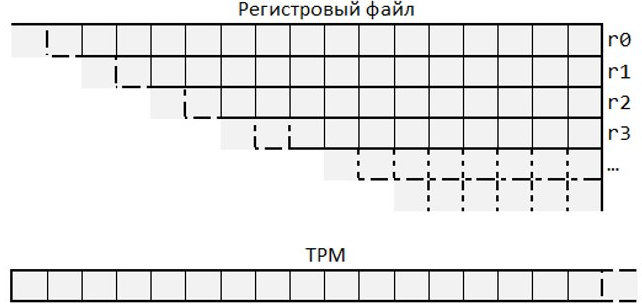
\includegraphics[scale=0.35]{Images/reg_and_tpm.png}
    \caption{Репрезентация регистрового файла и TMP.}
    \label{fig:mem}
\end{figure}

Векторный компилятор intel имеет возможность векторизовать и разложить на регистры последовательные типы данных. В них входят вектора, массивы, структуры, состоящие из элементов одного примитивного типа и так далее. Так, например, компилятор может обработать структуру type \{float, <7 x float>\} и преобразовать её в вектор <8 x float>. Однако, векторизация не справлялась с более сложными структурами. На Рис~\ref{fig:lying} видно, что структура S без поля int32\_t может быть оптимизирована, векторизована и положена на регистры. Но, как только появляется дополнительное поле иного типа, в данном случае это int32\_t, встаёт вопрос как векторизовать такой объединённый тип. Это приводило к использованию структур из памяти, появлению spilling'ов и, таким образом, к сильному падению производительности. Решение проблемы векторизации структур решит проблему размещения структур на регистры и сократит количество обращений в память.

\begin{figure}[ht]
    \centering
    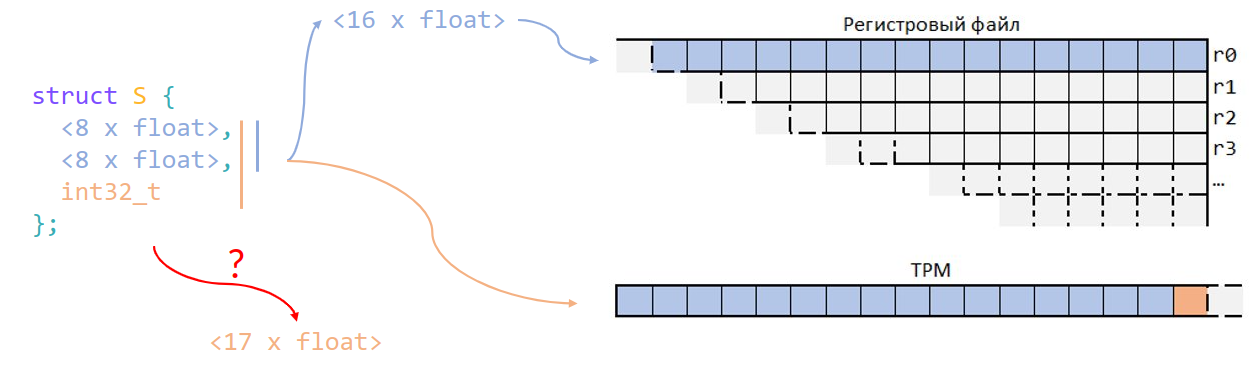
\includegraphics[scale=0.21]{Images/reg_and_tpm_lying.png}
    \caption{Возможное расположение структуры в памяти.}
    \label{fig:lying}
\end{figure}

%%
%%